\begin{figure*}
\begin{center}
\fbox{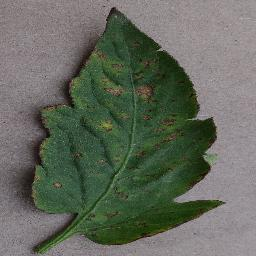
\includegraphics[scale=0.262]{./images/normal_3159}
	   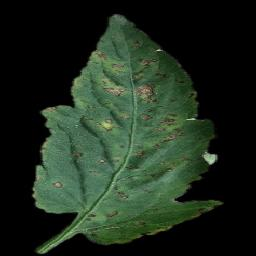
\includegraphics[scale=0.262]{./images/segmented_3159}
	   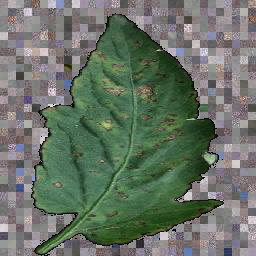
\includegraphics[scale=0.35]{./images/9_ROTATE_180_crop}
	   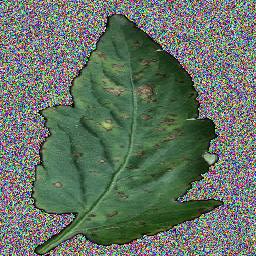
\includegraphics[scale=0.262]{./images/196_ROTATE_270}
	   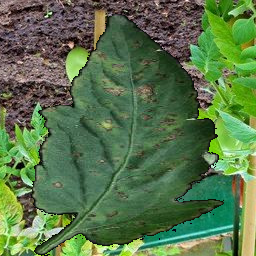
\includegraphics[scale=0.35]{./images/random_backgorund}
	   }
	\begin{center}
		\caption{Sampels of training images, from left to right: \textbf{Original PlantVillage dataset}, \textbf{Segmented PlantVillage dataset}, \textbf{Random background Crop dataset}, \textbf{Random Noise Backgorund} and \textbf{Random Background Image}}
		\label{fig:samples}
	\end{center}
	\vspace{-15pt}
\end{center}
\end{figure*}

\section{Experiments}
Our experiments are on two main task: Binary Classification, Multi-class Classification. In this section first we describe the dataset and the variations created to perform sensitivity analysis. Then we go trough the experiments setup were we describe how we have conducted the experiments to accomplish the two task and finally we show the results.

\subsection{Datasets}
We analyze 18158 images of tomato plant leaves, which are splitted in 10 classes, 9 diseases and 1 healthy. The scope is to predict the correct class of a leaf given its image. All the images are sized 256x256. 
\\\indent Given the original dataset we have conducted the training phase on different variations of the original dataset, we have worked on the background in order to find a way to overcome the limits highlined in \cite{} and confirmed by us.
In Figure \ref{fig:samples} we can see all the images the different versions of the dataset that we have tested and built.
\begin{itemize}
\item{\textbf{Original PlantVillage dataset} it consists of images of tomato leaves lain over a gray table.}
\item{\textbf{Segmented PlantVillage dataset} it consists of images of tomato leaves without the original background, this variation was used also in \cite{}. In our work we have re-segmented the images since in the available segmented dataset was not complete.}
\item{\textbf{Random Background Crop dataset} it consists of the leaf images coming from PlantVillage with a background composed of crops of background coming from the Original Plantvillage Dataset. We have tried this variation in order to exploit the dependence between original backgrounds and the class we found out in the experiment on the original dataset.}
\item{\textbf{Random Noise Backgorund} it consists of leaf images coming from PlantVillage with a background composed of random colored pixels. As before we tried this experiment to exploit the dependence between background and classes higlined in the original dataset.}
\item{\textbf{Random Background Image} it consists of leaf images coming form Plant Village with a background taken from a set of 4176 we built looking for tomato plantation images . The objective of this set was not only to exploit the backgorund influence on the classifier but also try to take the leaf in a situation similar to a realistic one, where the leaf image is taken directly in the plantation.}
\end{itemize}

\subsection{Experiments setup}
\subsubsection{Data Augmentation and Normalization}
As showed in Figure \ref{fig:1} after the Train-Test Split and Transformation Selection Phases our train set goes trough augmentation and normalization.
\\\indent We have performed data augmentation applying to the original sample two transformations from this pool:
Flip Top Bottom, 	Flip Left Right, Rotate 90\degree, Rotate 180\degree, Rotate 270\degree, Flip Top Bottom and Rotate 90\degree, Flip Top Bottom and Rotate 270\degree.
\\\indent After augmentation we have three samples for each original image (1 original image + 2 transformed images).
We have done this in order to train the networks with more data and strength the obtained model.
\\\indent Another key aspect of our setup is the normalization of the input images, the chosen normalization changes dramatically the validation accuracy. In our work we have explored the space of possible normalization considering these:
	\begin{itemize}
		\item{\textbf{Dataset Normalization} given the chosen variation of the dataset we have computed the mean and the standard deviation of the whole dataset.}
		\item{\textbf{Per-leaf Normalization} starting from the segmented dataset we have computed the mean and standard deviation of the non-black pixels.}
	\end{itemize}
\subsubsection{Binary Classification Setup}

\textbf{LeNet}
This network proposed in \cite{ref30} is one of the simplest deep model available. We have adapted it to perform our binary task. \\
\textbf{Weights Inizialization:}
for this network we started using training from scratch approach. The weights in the net are initialized using Xavier initialization \cite{ref31}. This helps training  since we start from a normally distribute set of weights and we avoid that certain weighs vanish trough epochs.
\\
\textbf{Activation Function:}
layers activation function is rectified linear unit (ReLU) since diminishes the likelihood of a gradient to vanish.
\\
\textbf{Loss Function:}
the chosen loss function for the binary classification is BCEWithLogitsLoss since it is designed for binary tasks and more stable compared to cross entropy.
\\
\textbf{Validation:}
for this task we have performed k-fold cross validation with k = 10 over the training set. This kind of validation was used to estimate the number of training epochs.
\subsubsection{Multi-class Classification Setup}
\textbf{AlexNet}
for this task we have chosen a more complex model since we have tested LeNet over the ten class with results very far from the state of the art \cite{ref11}. In order to compare our results with \cite{ref11} we have chosen AlexNet.  \\
\textbf{Weights Inizialization:}
for this network we have tried both training from scratch approach and transfer learning. \\\indent The weights in the first case are initialized using Xavier initialization \cite{ref31}. This helps training  since we start from a normally distribute set of weights avoids that certain weighs vanish trough epochs.\\\indent In the transfer learning approach we have used the weights coming from the training on ImageNet \cite{imagenet}.
\\
\textbf{Activation Function:}
layers activation function is again rectified linear unit (ReLU).
\\
\textbf{Loss Function:}
in this case we have used Cross Entropy as loss function.
\\
\textbf{Validation:}
in the case of Multi-class Classification we opt to proceed with cross validation. We have chosen a different approach from binary classification. In fact k-fold cross validation required on AlexNet requires a lot of computing time that is not justified in our dataset since there is small amount of variance in our pictures and consequently in each possible fold.
\\
\textbf{Optimizer:}
As optimizer we have choosen Adam \cite{ref32}. An important annotation should be done about this optimizer. In fact trough the training process we noticed that accuracy after a bunch of epochs drops. This was caused by the $\varepsilon$ coefficient, this coefficient used to avoid division by zero when the gradient is almost zero in parameters update.  By default is set to $1*10^{-8}$ and it causes large weights updates. So we set it to 0.1 to avoid this problem.
\subsection{Results and discussion:}
